\chapter{My First Chapter}
\blindtext \blindtext

Use abbreviation like this: \gls{1D}; use nomenclature like this: \gls{cp}.


\section{Itemization}
\begin{itemize}
\item Item 1
\item Item 2
\item Item 3
\end{itemize}


\section{Math equations}
Equation \ref{eq:compressor_volumetric efficiency} describes the volumetric efficiency for the compressor, where $\dot Q \textsubscript{real}$ is the measured volume flow rate generated by the compressor at the discharge port.

\begin{equation}
\label{eq:compressor_volumetric efficiency}
\eta \textsubscript{vol} = \frac{\dot Q \textsubscript{real}}{\dot Q \textsubscript{theory}} = \frac{\dot m \textsubscript{real}}{\dot m \textsubscript{theory}}
\end{equation}


\section{Citation/reference}
The Fiala Physiological Comfort (FPC) model \cite{fialaDynamicSimulationHuman1998} describes...


\section{Figure}
This is to test figure and table. In Figure \ref{fig:awesome_image} we showed a picture.
\begin{figure}[h]
\centering
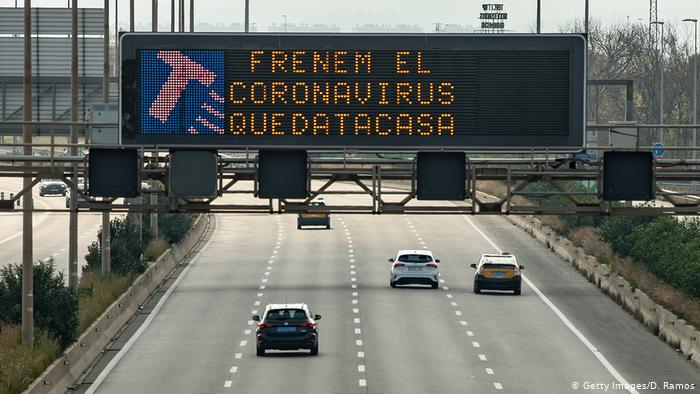
\includegraphics[width=0.8\textwidth]{52776268_303}
\caption{Awesome Image}
\label{fig:awesome_image}
\end{figure}

\section{Table}
In Table \ref{tab:my_awesome_table} we described the weather.

\begin{table}[h]
\centering
\caption{My Awesome Table}
\label{tab:my_awesome_table}
\begin{tabular}{ l l l p{2in} }
\hline
Day & Min Temp & Max Temp & Summary \\ \hline
Monday & 11C & 22C & A clear day with lots of sunshine.
However, the strong breeze will bring down the temperatures. \\ \hline
Tuesday & 9C & 19C & Cloudy with rain, across many northern regions. Clear
spells
across most of Scotland and Northern Ireland,
but rain reaching the far northwest. \\ \hline
Wednesday & 10C & 21C & Rain will still linger for the morning.
Conditions will improve by early afternoon and continue
throughout the evening. \\
\hline
\end{tabular}
\end{table}
